\documentclass[11pt, oneside]{amsart}   	% use "amsart" instead of "article" for AMSLaTeX format
\usepackage{geometry}                		% See geometry.pdf to learn the layout options. There are lots.
\geometry{letterpaper}                   		% ... or a4paper or a5paper or ...
%\geometry{landscape}                		% Activate for rotated page geometry
%\usepackage[parfill]{parskip}    		% Activate to begin paragraphs with an empty line rather than an indent
\usepackage{graphicx}				% Use pdf, png, jpg, or eps§ with pdflatex; use eps in DVI mode
								% TeX will automatically convert eps --> pdf in pdflatex
\usepackage{amssymb}
\usepackage{amsmath}
\usepackage{hyperref}

%SetFonts
\usepackage[utf8x]{inputenc}
\usepackage[T1]{fontenc}
\usepackage{lmodern}


\nonstopmode
%----macros begin-----------------------------------------------------------------------------------
\usepackage{graphicx}
\usepackage{color}

\def\conv{\mbox{\textrm{conv}\,}}
\def\aff{\mbox{\textrm{aff}\,}}
\def\B{\mathbb{B}}
\def\N{\mathbb{N}}
\def\E{\mathbb{E}}
\def\R{\mathbb{R}}
\def\Z{\mathbb{Z}}
\def\v#1{{\bf #1}}
\def\p#1{{\bf #1}}
\def\T#1{{\bf #1}}
\def\vet#1{{\left(\begin{array}{ccccccc}#1\end{array}\right)}}
\def\mat#1{{\left(\begin{array}{ccccccc}#1\end{array}\right)}}

\def\lin{\mbox{\rm lin}\,}
\def\aff{\mbox{\rm aff}\,}
\def\pos{\mbox{\rm pos}\,}
\def\cone{\mbox{\rm cone}\,}
\def\conv{\mbox{\rm conv}\,}

%----macros end-----------------------------------------------------------------------------------


% rules for for inputed tables
% the
\usepackage{siunitx}
\usepackage{booktabs}

%alternative rules for tables
%\newcommand{\toprule}{\hline}
%\newcommand{\midrule}{\hline}
%\newcommand{\bottomrule}{\hline}
%\newcommand{\specialrule}{}

%SetFonts



\title{Algebraic filtering of surfaces from medical images with Julia}
\author{Miroslav Jirik and Alberto Paoluzzi}
\date{}							% Activate to display a given date or no date

\begin{document}
\maketitle

\begin{abstract}
In this paper we introduce a novel algebraic \textsc{lar-surf} filter, well founded on algebraic topology methods, to extract and smooth the boundary surface of any subset of voxels arising from  segmentation of a 3D medical image. The input is defined as a \emph{chain}, i.e.~as a vector from a linear space of 3-chains, represented in coordinates as a sparse binary vector. The output is produced by a linear mapping between spaces of 3- and 2-chains through the boundary operator $\partial_3:C_3 \to C_2$.  In particular, when the input set of voxels is either not (4-)connected, or contains one or more empty regions inside, \textsc{lar-surf} generates a non connected set of closed surfaces, i.e.~a set of 2-cycles---using the language of algebraic topology. The only data structures used by this approach are sparse arrays with one or two indices, i.e.~sparse vectors and matrices. This work is based on LAR (Linear Algebraic Representation) methods, and is implemented in Julia language, natively supporting parallel computing on hybrid architectures.
\end{abstract}

\tableofcontents

%\section{}
%\subsection{}

\section{Introduction}\label{sec:intro}


Isosurface extraction produces geometric model of surface 
 from volumetric data is important in many aplications. It is often used for indirect visualization of the medical data or for flow modeling \cite{Rohan2018a}.
 
 
The most popular algorithm used for surface extraction is probably Marching Cubes (MC). The algorithm was described by Lorentsen and Cline \cite{Lorensen1987} in 1987. Survey of Marching Cubes algorthm has been published in 2006 \cite{Newman2006}. The algorithm is based on considering the cube defining volume. Each corner vertex of the cube is related to input volumetric data. MC traverse the data and constructs the surface by using lookup table of different triangular faces depending on different patterns of the cube.  Main disadvantages of this method are time requirements, ambiquity and holes generation. Some of them were discoverd shortly after the algorithm was introduced. 
Marching Cubes. In 1991 Nielson and Hamman described Asymptotic Decider to solve the ambiguity problem on the faces of the cube.  Natarajan noted that the ambiguity problem also occurs in cubes \cite{Natarajan1994}. In 1995 Chernyaev extended the number of cases to 33 \cite{chernyaev1995marching}. More recently the algorithm was updated by Custodio to   enhance the quality of triangulation \cite{Custodio2019}. 

The alternative methods have been deveoloped including method for surface extraction using particle attraction system was described by Crossno and Angel in \cite{Crossno2002} and method processing on a graph that tracks cell face adjacencies is described in \cite{Lachaud2000}. The parallel algorithms for surface extraction are discussed in \cite{Bajaj2004}.





\section{Background}\label{sec:background}


\subsection{Representation Schemes}\label{sec:aaaa}

A \emph{representation scheme} for solid modeling is a mapping between a space of mathematical models and a space of symbolic representations, like generated by a formal grammar.
Solid pointsets (i.e., `$r$-sets') are defined~\cite{Requicha:1980:RRS:356827.356833} as compact (bounded and closed) regular and semianalytic subsets of the $d$-space. A large number of representation schemes were defined in the past forty years, including the two main classes of (a) \emph{boundary representations} (`$B$-reps'), where the solid model is represented through a representation of its boundary elements, i.e.~faces, edges and vertices, and (b) \emph{decompositive/enumerative representations}, that are a decomposition of either the object or the embedding space, respectively, into a well-defined \emph{cellular complex}. In particular, a boundary representation provides a cellular decomposition of the object's boundary into \emph{cells} of dimension zero (vertices), one (edges), and two (faces). Medical imaging can be classified as \emph{enumerative representation} of cellular decompositions of organs and tissues of interest, in particular, as subsets \emph{of 3D volume elements} (voxels) from the 3D image. 


\subsection{Linear Algebraic Representation}\label{sec:aaaa}

The \emph{Linear Algebraic Representation} (\textsc{lar})~\cite{Dicarlo:2014:TNL:2543138.2543294} aims to represent the \emph{chain complex}~\cite{TSAS} generated by a piecewise-linear \emph{geometric complex} embedded either in 2D or in 3D. In few words, it gets a minimal characterization of geometry and topology of a cellular complex, i.e.~the embedding mapping $\mu : C_0 \to \E^d$ of 0-cells (vertices), as well a description of $(d-1)$-cells as subsets of vertices, and is able to return the whole chain complex 
\[ 
C_\bullet = (C_p, \partial_p) := 
C_3 \ 
\substack{
\delta_2 \\x
\longleftarrow \\[-1mm]
\longrightarrow \\
\partial_3 
}
\ C_2 \ 
\substack{
\delta_1 \\
\longleftarrow \\[-1mm]
\longrightarrow \\
\partial_2 
}
\ C_1 \ 
\substack{
\delta_0 \\
\longleftarrow \\[-1mm]
\longrightarrow \\
\partial_1 
}
\ C_0 .
\] 
and, in particular, any basis for linear chain spaces $C_p$, and any linear
boundary/coboundary map \(\partial_p\) and
\(\delta_p=\partial_{p-1}^\top\) between them. The \emph{domain} of \textsc{lar} is the set of \textbf{chain complexes} generated by cell $d$-complexes ($2\leq d\leq 3$). The computer \emph{representations} of \textsc{lar} are \textbf{sparse binary matrices} to represent both the operators and the chain bases. Note that in algebraic topology a $p$-chain is defined as a linear combination of $p$-cells with scalars from a field. When the scalar coefficients are from $\{-1, 0, +1\}$, a chain may represent \emph{any (oriented) subset of cells} from the cellular complex. 

We may therefore get the $(p-1)$-boundary $\partial_p c_p$ of \emph{any} $p$-chain $c_p$, by multiplication of the coordinate representation $[\partial_p]$ of the boundary operator times the coordinate representation $[c_p]$ of the chain in terms of such scalars, i.e.~by a  matrix-vector product $ [\partial_p] [c_p] $.

It is possible to show that the \textsc{lar} representation scheme is very expressive, i.e.~that it  has a large domain,  including collections of: line segments, quads, triangles, polygons, meshes;  pixels, voxels, volume images; B-reps, enumerative and decompositive representations of solids. 
In this paper we apply \textsc{lar} methods to computation of boundary representations of solid models from segmentation (labeling) of 3D medical images.
To display a triangulation of  boundary faces  in their proper position in space, the information required is contained in the \emph{geometric chain complex} (GCC):
\[
\mu: C_0\to\E^3,\ (\delta_0, \delta_1, \delta_2)
\qquad\equiv\qquad
\texttt{(geometry, topology) = (W, (EV, FE, CF))}
\]
The GCC allows to transform the (possibly non connected) boundary 2-cycle of surfaces as a standard B-rep~\cite{shapiroSM:202}. 
The \texttt{geometry} is given by
the embedding matrix \texttt{W} of vertices (0-cells), and \texttt{topology} is
given by the three sparse matrices \texttt{CF}, \texttt{FE}, \texttt{EV} of coboundaries
{i.e.},~$\delta_3, \delta_2, \delta_1$, of  chain complex describing a   
space arrangement~\cite{paoluzzi2019finite}.
Note that ordered pairs of letters from \texttt{V,E,F,C}, correspond to \emph{\emph{\texttt{V}}ertices$\to$\emph{\texttt{E}}dges$\to$\emph{\texttt{F}}aces$\to$\emph{\texttt{C}}ells} into the 
\emph{\emph{\texttt{C}}olumn$\to$\emph{\texttt{R}}ow} order of matrix maps of operators.



\subsubsection{Construction of boundary matrix $\partial_d$}

Once fixed an ordering for all the cells (vertices, edges, pixels, and voxels), i.e.~for 0-, 1-, 2-, and 3-elements of a cell partition \texttt{V,E,F,C} of a 3D image, i.e., once fixed the $p$-bases for linear spaces $C_p$ of $p$-chains $(0\leq p\leq 3)$, we call $M_p = (m_{i,j})$ the \emph{characteristic matrix} of the $p$-basis, expressed as subsets of 0-cells, where  we have that $m_{i,j}=1$ iff the $j$-th $0$-cell belongs to the boundary of $i$-th $p$-cell, and $m_{i,j}=0$ otherwise.  

Note that, by computing the (sparse) matrix product $(M_{p-1} M_{p}^t) = (n_{i,j})$, with $n_{i,j} = \sum_{k} m_{i,k}m_{k,j}$, we get for each $n_{ij}$ the \emph{number of vertices} shared by $c_{p-1}^i$ and $c_{p}^j$. When this number equates the cardinality of $c_{p-1}^i$, this elementary chain is contained on the boundary of $c_{p}^j$. In a 3D image, with cubic 3-cells and squared 2-cells in between, everywhere we get $n_{i,j}=4$, we may state $c_{2}^i\subset\partial c_{3}^j$. In this case, by looking in each $j$ column of $M_{2} M_{3}^t = (n_{i,j})$, we have exactly \emph{six rows} where  $n_{i,j} = 4$. 

Finally, consider the linear graded boundary operator $\partial_p : C_p \to C_{p-1}$. As such, it contains by columns the representation of domain basis elements, expressed as linear combination of the basis elements of the range space. Therefore, the operator matrix $[\partial_d]$ is readily obtained by setting $[\partial_d](i,j)=1$ iff $n_{i,j}=4$ and $[\partial_d](i,j)=0$ otherwise.  Of course, it will contain six non-zero elements for column.  It may be worth to remember that every 3-cell (voxel) of 3D image has exactly six 2-faces. 

It is possible to show that all the interesting relations of incidence/adjacency between cells of different dimensions can be both computed and efficiently queried by pairwise computing some matrix products, with one of terms possibly transposed, using only the two boundary and coboundary operator matrices $[\partial_p]$ and $[\delta_p]$, and where $[\delta_p] = [\partial_p^\top]$. We~may also show that such matrices are \emph{very sparse}, with their sparseness growing rapidly with the dimensions (see Section~\ref{sec:block}). The pattern of non-zeros in matrix $[\partial_3]$ corresponding to a brick of shape $(4,4,4)$ is given in Figure~\ref{fig:boundary_matrix_4x4x4}.

\begin{figure}[htbp] %  figure placement: here, top, bottom, or page
   \centering
   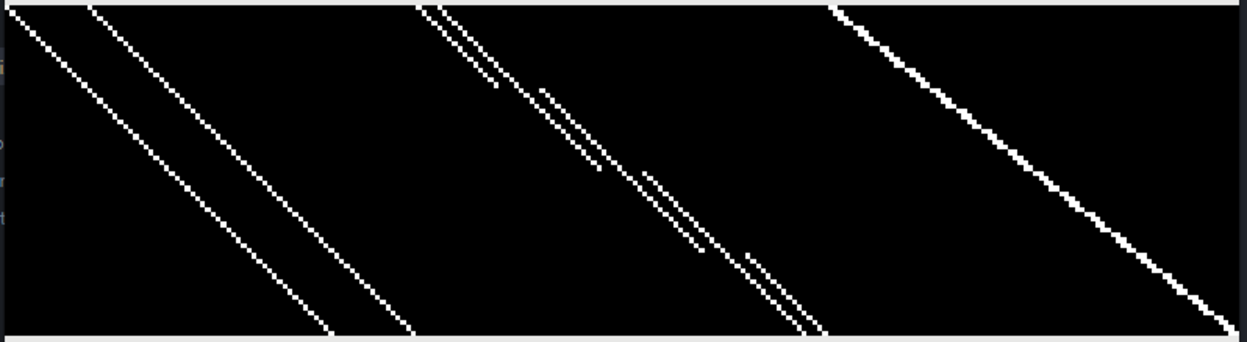
\includegraphics[width=0.75\linewidth]{figs/boundary_matrix_4x4x4.pdf} 
   \caption{A binary image of the coboundary operator  $\delta_2 = \partial_3^\top : C_2 \to C_3$, built for a small 3D image with shape $(4,4,4)$. Note that the number of rows equates the cardinality $4\times 4\times 4 = 64$ of the voxel set; the number of columns is $d\,n\,(1+n)^{d-1} = 3\times 4\times 25 = 300$. Of course, the number of non-zeros per row (cardinality of single voxel facets) is six, whereas the number of non-zeros per column is two, but on boundary facets.}
   \label{fig:boundary_matrix_4x4x4}
\end{figure}

\subsection{Multiindices from Cartesian indices}\label{sec:aaaa}

In order to utilize the topological algebra shortly recalled in this paper, we need to explicitly sort the cells of the various dimensions into linearly ordered sequences, possibly according to the linear order their information is linearly accommodated in computer storage. 

\subsection{Taubin Smoothing}\label{sec:aaaa}






\section{Block-parametric design}\label{sec:filter}

\subsection{Block decomposition}\label{sec:bbbb}

We assume that medical devices produce 3D images with lateral dimensions that are integer multiples of some powers of two, like 128, 256, 512, etc.
Any cuboidal portion of image is completely determined by the Cartesian indices of its voxels of lowest and highest indices, and extracted by multidimensional array \emph{slicing} as $Image([\ell_x$:$h_x, \ell_y$:$h_y, \ell_z$:$h_z])$.

For the sake of simplicity, we assume a common size on the three image axes, and the corresponding image portion $\B$, called \emph{block}, as a function of its element of the  lowest  block  coordinates $i,j,k\in [1:n]$ and of block dimension $n\in\N$:
\[
\B(i,j,k,n) := Image([in:in+n, jn:jn+n, kn:kn+n]) 
\]

\begin{figure}[htbp] %  figure placement: here, top, bottom, or page
   \centering
   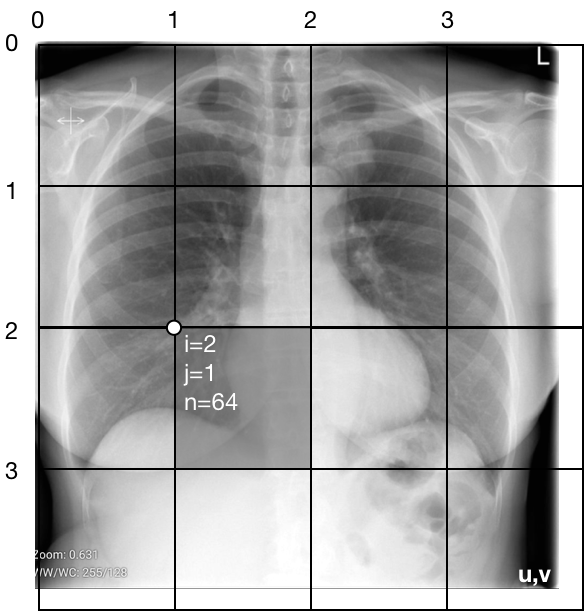
\includegraphics[width=0.5\linewidth]{figs/blocks} 
   \caption{A possible block partitioning of a radiologic image. The evidenced 2D block, of size $n^d=64^2$, is sliced by $\B([2,1,64]) = Image([128:172],[64:128)]$}
   \label{fig:blocks}
\end{figure}


Figure~\ref{fig:blocks} shows the block decomposition in a 2D image, with positive integers $(u,v)$ giving the lateral sizes of image. Note that block sides do not necessarily correspond to image edges. 


\subsection{Block operator }\label{sec:block}

\paragraph{Chain coordinates }\label{sec:bbbb} 
We are going to treat each image block independently from each other. Hence we map each image subspace $\B(i,j,n)$ to the linear \emph{chain} space $C_2$ of dimension $n\times n$, using coordinate vectors $c_{h,k}\in \\B^{n\times n} := \{0,1\}^{n\times n}$, where the basis element $c = c_{h,k} \in C_2$ is mapped via Cartesian-to-linear map to the binary vector 
\[
Image(h,k) \mapsto c_{h,k} := [0 \cdots 0\ 1\ 0 \cdots 0] \in \B^{n\times n}
\]
for each $0\leq h,k \leq n$, and where the (single) unit element is in position $nk + h \leq n\times n$.

Therefore, each pixel (or voxel) in a block image will be seen as a basis binary vector in $C_2$, and each subset of image elements, as the corresponding binary vector in $C_2$, with many ones as the cardinality of the subset.

\paragraph{Boundary operator }\label{sec:bbbb} For a fixed block size $n$, the boundary operator $\partial_d : C_d\to C_{d-1}$, with $d\in\{2,3\}$, will be constructed once and for all using the algorithm given in~\cite{}, and inlined in the generated boundary extraction code.

It is easy to see that the operator's matrix $[\partial_d]$ is \emph{very sparse}, since it contains $2\times d$ non-zero elements (ones) for each column (of length $n^d$), i.e.~4 ones and 6 ones for the 2D and 3D case, respectively. In fact the matrix of a linear operator between linear spaces contains by columns the basis element of the domain space, represented in the target space. In our case, the former is an image element (2-cube or 3-cube), represented as the chain of its boundary---i.e. either a 1-cycle of 4 edges, or  a 2-cycle of 6 faces, respectively.  

The number of rows of $[\partial_d]$ equates the dimension of the linear space $C_{d-1}$, i.e.~the number of $(d-1)$-cells---elementary $(d-1)$-chains---in the cellular partition of the image. To compute their number, we act in two steps. (a) First we map one-to-one the $n^d$ $d$-cells with $d$ adjacent $(d-1)$-cells, so getting $d\,n^d$ distinct basis elements of $C_{d-1}$. (b) Then we complete this bases by adjoining $n^{d-1}$ boundary elements for each of the $d$ dimensions of the image, so providing further $d\,n^{d-1}$ basis elements for $C_{d-1}$. The dimension of $C_{d-1}$, and therefore the number of rows of $[\partial_d]$ matrix is $d\,(n^{d-1}+n^{d}) = d\,n\,(1+n)^{d-1}$. The number of column equates the number of basis elements of $C_d$, i.e.~the number $n^d$ of block elements.

\paragraph{Sparsity and size of boundary matrix }\label{sec:bbbb} 

As we have seen, we have $2d$ non-zero elements for each column of $[\partial_d]$, so that their total number is $2d\,n^d$. The number of matrix element is $d\,n\,(1+n)^{d-1} \times n^d$, giving a ratio of 
\[
\frac{\mbox{non-zero\ elements}}{\mbox{total\ elements}} = 
\frac{2d\times n^d}{d\,n\,(1+n)^{d-1} \times n^d} =
\frac{2}{n+n^d}
\]
Using sparse matrices in CSC (Compressed Sparse Column) format we get a storage size:
\[
mem([\partial_d]_{n^d}) = 2\times \#\mbox{nzero} + \#\mbox{columns} = 2\times 2d\,n^d + n^d = (4d+1)n^d.
\]
In conclusion, for block size $n=64$, the matrix $[\partial_d]$ requires for 2D images $9\times 64^2=36,864$ memory elements, and for 3D images $13\times 64^3=3,407,872$ memory elements. Counting the bytes for the standard implementation of a sparse binary matrix (1 byte for values and 8 bytes for indices) we get $(18d+8)n^d$ bytes, giving $176$\,KB for 2D and $15.872$\,MB for 3D.


\begin{figure}[htbp] %  figure placement: here, top, bottom, or page
   \centering
   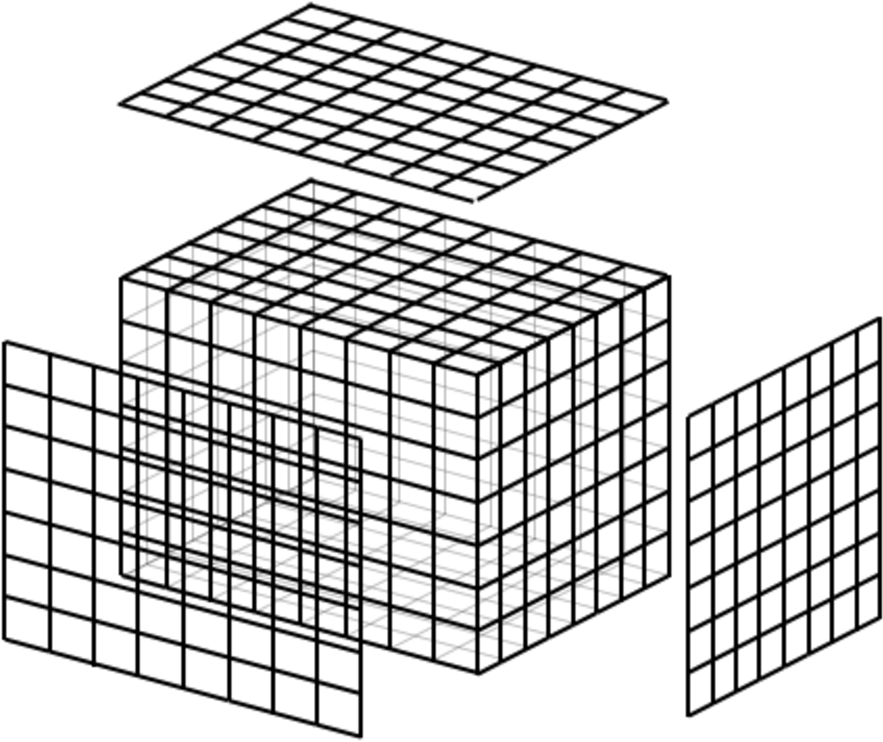
\includegraphics[width=0.4\linewidth]{figs/grid.pdf} 
   \caption{example caption}
   \label{fig:example}
\end{figure}



\subsection{Block boundary mapping}\label{sec:bbbb}

Here we refer directly to the 3D case.
Let us call \emph{segment} the bulk content $S$ of interest within the input 3D image of size $(u,v,w)$. We aim to compute the segment boundary $\partial_3 S$. 
First we set the size $n$ of the block, in order to decompose the input $Image(u,v,w)$ into a fair number 
\[
M = \ceil{u/n} \times \ceil{v/n} \times \ceil{w/n} \simeq \frac{uvw}{n^3}
\] of blocks. 
Then we consider each image portion $c_{i,j,k} = S\cap \B(i,j,k,n)$ and compute its (binary) coordinate representation  $[c]_{i,j,k}\in C_3(n,n,n)$. This one is a sparse binary vector of length $n^3$. Then assemble the $M$ representations $c$ of segment portions into a sparse binary matrix $\T{S}$, of dimension $n^d \times M$. Finally compute a matrix $\T{\B}$ of boundary portions of $S$, represented by columns as chain coordinate vectors in $C_2$:
\[
\T{\B} = [\partial_3(n)]\, \T{S}.
\]
where the boundary matrix has dimension $d\,n\,(1+n)^{d-1} \times n^d$.
Of course, the $\T{\B}$ sparse matrix has the same column number $M$ of $\T{S}$, because each column contains the boundary representation of the corresponding $S\cap Box_{i,j,k}{i,j,k}$, and the number of rows of the operator, equal to the dimension of the linear space $C_2$.

\paragraph{Embedding}
A final computational step is needed, in order to embed the 2-chains in Euclidean space $\E^3$ and to assemble the whole resulting surface. In particular, we need to compute the \emph{embedding function} $\mu : C_0 \to \E^3$, where $C_0$ is the space of 0-chains, one-to-one corresponding to the vertices of the extracted surface. The simplest solution is to associate  four 0-cells to each 2-cell of the extracted surface, i.e.~to each non-zero entry in every column of $\T{\B}$.  The $\mu$ function  can be computed by identifying, via  element position in the column, a triple of integer values $0\leq x\leq u$, $0\leq y\leq v$, and $0\leq z\leq w$ for each vertex of the 2-cell.  The mapping can be implemented using a dictionary, that will store the inverse coordinate transformation used at the beginning, i.e.~the one from linear to Cartesian coords, in order of not duplicating the output vertices.   

\paragraph{Surface assembling}

All boundary surface subsets $\B_{i,j,k}(S) = \partial_3 S \cap \mbox{Box}_{i,j,k}$, provided by  columns of $\T{S}$, are embedded in the same coordinate space. In formal terms: 
\[
\texttt{Lar}(S) := (\texttt{Geom}(S), \texttt{Top}(S)) = (\texttt{V}, \texttt{CV}),
\]
where, with respect to the \emph{chain complex} $C_3\to C_2\to C_1\to C_0$ induced by the input image $Im$ and segment $S_{i,j,k}$, we get
\begin{align}
\texttt{Geom} &:= \mu(C_0(_{i,j,k})) = \texttt{V},
\\
\texttt{Top} &:= C_3(S) = \T{S} \mapsto \texttt{CV}.
\end{align}
and
\begin{align}
\texttt{Lar}(B_{i,j,k}) &:= (\texttt{Geom}, \texttt{Top}) = (\texttt{W}, \texttt{FW}),
\\
\texttt{Geom} &:= \mu(C_0(B_{i,j,k})) = \texttt{W} \subset \texttt{V},
\\
\texttt{Top} &:= C_2(B_{i,j,k}) = \T{\B}_{i,j,k} \mapsto \texttt{FW} \subset \texttt{FV}.
\end{align}


A translation transformation applied to each vertex subset $\texttt{W}_{i,j,k}$ with translation  vector $\v{t} = [i,j,k]$ will therefore move it in the final space position, so finally giving
\[
\texttt{Lar}(\B) = \oplus_{i,j,k}\texttt{Lar}(\partial_3 S_{i,j,k})) = \oplus_{i,j,k}(\texttt{W}, \texttt{FW}) .
\]


\subsection{Block-level parallelism}\label{sec:bbbb}

In the computational pipeline introduced in this paper, several steps can be efficiently performed in parallel at image-block level, depending on the embarassingly data parallel nature of the problem. In particular, little effort is needed to separate the problem into a number of parallel tasks $S_{i,j,k}$, using multiarray slicing. The granularity of parallelism, depending on the block size $n$, is further enforced by the computation of a single boundary matrix $[\partial_d(n)]$, in turn depending on $n$, so that the initial communication cost of broadcasting the matrix to nodes can be carefully controlled, and finely tuned depending on the system architecture. The whole approach is appropriate  for SIMD hybrid architectures of CPUs and GPUs, since only the initial block setup of boundary matrix and image slices, as well the final collection of computed surface portions, require inter-process communication.






\section{Julia implementation}\label{sec:implementation}

The computer code is implemented in Julia language~\cite{} according to the workflow described below, whose stages are parallelized and/or optimized in various ways.

\subsection{Parallel workflow}\label{sec:implementation}


\paragraph{Workflow setup} The functions in this preliminary step include:
\begin{enumerate}

\item input of 3D medical image $\mathcal{I}$ dimensions $\ell_1, \ell_2, \ell_3$, such that: $\mathcal{I} = [\ell_1]\times[\ell_2]\times[\ell_3]$, where $[\ell_k] = (1,2,\ldots,\ell_k)$;

\item analysis of resources available in the computational environment, including operating system, type and number of compute nodes (processors, cores, GPUs), number of cores per node, RAM and caches amounts;

\item depending on the above, best decision for $\emph{size}$ of 3D image blocks $\mathcal{B}$ (bricks); defaults to: $\emph{size}=64$; hence the number of bricks will be $n=\ceil{\ell_1/size}\times\ceil{\ell_2/size}\times\ceil{\ell_3/size}$. 
Hence default value: $n=256$, for images $\mathcal{I} = 512\times 512\times 256$;

\item computation of a Julia's sparse boundary matrix $[\partial_B]$, returning a value of type \texttt{SparseMatrixCSC\{Int8\}\{Int64\}}, where \texttt{Int8} and \texttt{Int64} are the types for values and indices, respectively, stored by Compressed Sparse Column (CSC) format; the average $[\partial_B]$ (for $\emph{size}$ = 64) is about 45 MB;

\item creation of either a local or distributed channel to implement a producer/consumer model of parallel/distributed computation, depending on available resources;

\item distribution of matrix $[\partial_B]$, of default size $45$ MB, to all available nodes/cores (workers) using the macro \texttt{@eveywhere}. 

\end{enumerate}

The memory occupancy of the sparse matrix is computed by considering $8+1$ bytes for non-zero element (which are exactly 6 per row), plus 8 bytes per each index of column start.  
With $size=64$, the number of non-zeros within the sparse matrix $[\partial_{64^3}]$ is $\mathtt{nnz} = 4 792 266$, for a storage size of $9\times \mathtt{nnz}+8\times 262144 \simeq 45$ MB. 

\begin{figure}[htbp]
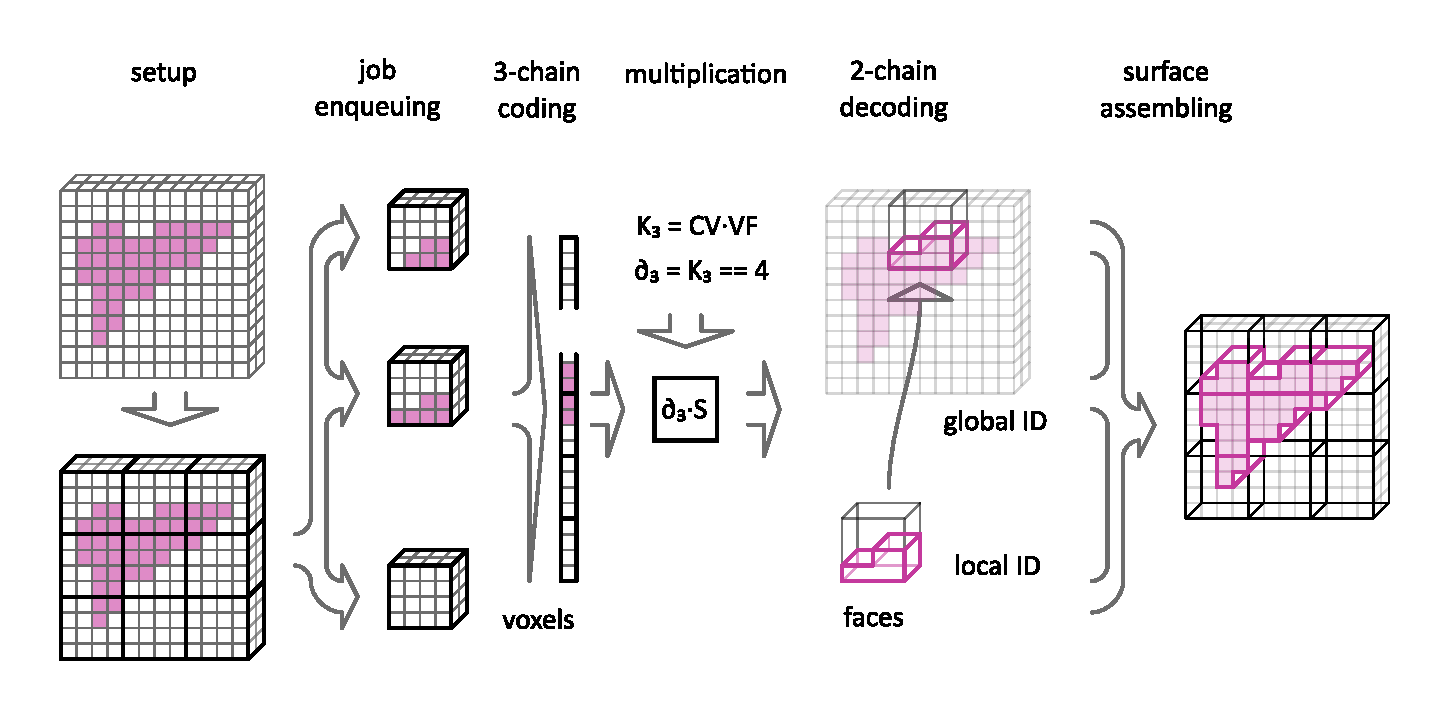
\includegraphics[width=0.99\textwidth]{figs/schema_horizontal.pdf} 
%\includegraphics[scale=1]{input/ircad_comparison.pdf} 
\caption{Workflow of LAR-SURF algorithm}
\label{fig:schema}
\end{figure}

With $size=64$, the number of non-zeros within the sparse matrix $[\partial_{64^3}]$ is $\mathtt{nnz} = 4 792 266$, for a memory size of $9\times \mathtt{nnz}+8\times 262144 \simeq 45$ MB. The memory size of the sparse matrix is computed by considering $8+1$ bytes for non-zero element (which are exactly 6 per row), plus 8 bytes per each index of column start.  


\paragraph{Job enqueuing} Communication and data synchronization may be managed through \emph{Channels}, which are the FIFO conduits that may provide producer/consumer communication. Overall execution time can be improved if other tasks can be run while a task is being executed, or while waiting for an external service/function to complete. The single work items of this stage follow:
\begin{enumerate}

\item extraction, from image arrays of the block views, depending on 3 Cartesian indices;

\item transform  each block \emph{from global} $[\ell_1]\times[\ell_2]\times[\ell_3]$ to \emph{local coordinates} $[n]\times[n]\times[n]$;

\item further transform of each \emph{foreground voxel} $\nu\in\mathcal{S}\subseteq\mathcal{I}$ from Cartesian to linear coordinates, using the suitable Julia's library functions.

\item enqueing the job (as a sequence of integer positions for the non-zeros image elements aligned in a memory buffer of proper \texttt{Channel} type).
\end{enumerate}

\paragraph{3-Chain encoding} 
The interesting part of the \emph{Image} $\mathcal{I}$ is called \emph{Segment} $\mathcal{S}$. The goal of the whole \emph{workflow} is to extract a \emph{boundary model} of $\mathcal{S}$ from $\mathcal{I}$. The portion of $\mathcal{S}$ inside $\mathcal{B}$, will be denoted as $\mathcal{S}(B)$.
Each block $\mathcal{B}$ of the 3D image must by converted into the \emph{coordinate representation} of a vector $\nu\in C_3$ in the linear space  of 3-chains. 

In coordinates local to $\mathcal{B}$, once fixed an ordering from Cartesian to linear coords, this vector is represented by a \emph{binary array} of length $size^3$. With $size=64$, we have $64^3=262144$,  with a non-zero value (i.e.~$1$) for each foreground voxel in $\mathcal{S}(B)$. Therefore, the coded segment portion $\mathcal{S}(B)$, results with a space occupancy of about $262$ KB if encoded as a full array (i.e.~including the zero values). Whether encoded as a sparse vector, its space occupancy will correspondingly decrease.

\begin{enumerate}

\item each encoding task produces either a full or sparse binary vector. With full or sparse arrays depending by one index, we get either 262 KB or less per job, correspondingly;

\item special format for sparse CSC (Compressed Sparse Column) vectors can be used, since the \emph{value} data for non-zeros does not need storage. Hence only a single 1-array of \texttt{Int64} row positions (with total length equal to the number of non-zeros in the block, with $8\times\mathtt{nnz}$ kB storage) is needed;

\item prepare subsequences of such data vectors (non-zero linear row indices), in order to feed efficiently the available processor threads.
In case of presence of one/more GPUs, a smaller size of the block---and hence of the boundary matrix and the encoded 3-chain vectors---and then much higher vector numbers, are preferable for speed.

\end{enumerate}

\paragraph{SpMM Multiplication} 
According to the current literature~\cite{} it is more convenient to execute SpMV (sparse matrix-vector) multiplications than SpMSpV (sparse matrix-sparse vector) multiplications. Since we have 256 such jobs (one multiplication per block) to perform in the standard setting of the algorithm\footnote{
Size of block $64^3$; size of image $512^2\times 256$.
}, or more in case of either smaller blocks or image greater than the standard one, this stage must be evidently parallelized and carefully tuned, possibly by using the GPU, if available.
\begin{enumerate}

\item Various multiplication algorithms are being experimented, using several packages for sparse linear algebra and/or custom implementations;

\item the total speed of this stage will strongly depend on the hardware available, on the granularity of blocks, and on the choice between dense/sparse storage of encoded 3-chains;

\item anyway, the compute elements or threads will be feed without solution of continuity in a \emph{dataflow} process. This parallel operation is, according to our preliminary experiments, the critical one of the whole workflow, in the sense that any $\Delta T$ (either positive or negative) in this stage will contribute to the total time $T$.

\end{enumerate}

\paragraph{2-Chain decoding} 
Each multiplication of $[\partial_B] : C_3 \to C_2$, times a 3-chain $\nu\in C_3$, produces a 2-chain  $\sigma\in C_2$, i.e.~the \emph{coordinate representation} of the \emph{boundary vector} $\sigma\in C_2$.  The inverse of the coding algorithm is executed in the present stage.  This process can also be partially superimposed in time with the previous ones, depending on the size of the memory buffers used to feed the CPU cores or the GPUs and get their results. Some elementary steps follow:

\begin{enumerate}

\item conversion from position of ones (or non-zeros) in the 2-chain to linear indices of rows;

\item conversion from linear indices to Cartesian indices in coordinates local to the $\mathcal{B}$ block, using the appropriate library functions;

\item conversion from each Cartesian index value to a suitably oriented (i.e.~with proper attitude) geometry quadrilateral (or pair of triangles) in local coordinates.

\end{enumerate}

A Julia's vectorized pipeline dataflow seems the more appropriate implementation model for the job of each worker.

\paragraph{Assembling and artifact filtering} 
The results of the previous stages can be described as a \emph{collection of sets} of \emph{geometric quadrilaterals (quads)}, each one encoded as an array of quadruples of integer indices, pointing to the linear array of grid vertices associated to the image block $\mathcal{B}$.  In other words, \emph{all quads} of \textbf{each job} are now given in the \textbf{same} \emph{local coordinates}.  Besides to put each partial surface $\mathcal{S}(B) = (\texttt{V}_B, \texttt{FV}_\sigma)$ in the global coordinate system of the image, the present stage must eliminate the redundant boundary features possibly generated at the edges of the partial surface $\mathcal{S}(B)$ within each block $\mathcal{B}$ such that $B \cap \mathcal{I} \not= \emptyset$:
\begin{enumerate}

\item translate each array $\mathtt{FV}_\sigma$, of type \texttt{Lar.Cells}, by summing to each vertex index the linearized offset of the Cartesian coordinates $(n,m,p)(B)$ of the $\mathcal{B}$'s \emph{reference vertex}, i.e.~the one with (all) lowest \emph{Cartesian coordinates} within the $\mathcal{B}$ block.

\item remove both instances of \emph{double quads} generated by \texttt{Lar} software at the block boundaries (see Figure~\ref{fig:blockboundary}). They are artifacts generated by the decomposition of the whole image into a number of blocks of tractable size.

\item 
a smart strategy of removal of such artifacts may be used, which does not require any sorting nor searching on the assembled array of quads. It will consist in arranging each block with all three dimensions decreased-increased by one, so that each 2-adjacent pair of blocks will be covering each other for a full side extent of blocks of depth one. The details of this \emph{artifact filtering} are elucidated in Section~\ref{sec:covering}.

\end{enumerate}

\paragraph{Smoothing} 
The final smoothing of the generated surfaces cannot be performed block-wise, since this would introduce smoothing artifacts at the block boundaries. Anyway, the Taubin smoothing~\cite{} can be performed in parallel, since for each vertex in the final surface (except eventually the ones on the image $\mathcal{I}$ boundaries) it essentially consist in computing a new position as a proper average of its neighborhood vertices, i.e.~by applying a discrete Laplacian operator.  Some appropriate set workers may so be assigne the task of generating iteratively a new position for the vertices they take cure of. In particular, we have:
\begin{enumerate}

\item Job enqueuing, by writing sets of integers (global linear indices of vertices) in array buffers of appropriate type \texttt{Channel};

\item iterated vectorized computation of proper averages of closed vertices;

\item job dequeuing, by recovering finished tasks from a channel and assembling the results into the embedding function $\mathtt{V}: C_0 \to \E^3$ providing an array of type \texttt{Lar.Points} of \texttt{Float64 $\times$ 3}, with vertex coordinates by column.
\end{enumerate}



\subsection{Performance analysis}\label{sec:analysis}

The size of boundary matrix is critical parameter of LAR-SURF method. To determine optimal size of boundary matrix the experiment on artifical data was performed (Fig.  \ref{fig:bm_size_tesla}). Size of experimental data is set to $512\times512\times512$ and it is derived from typical size of Computed Tomography medical images. Computation is done on Tesla DGX-1 machine.

\begin{figure}
\centering
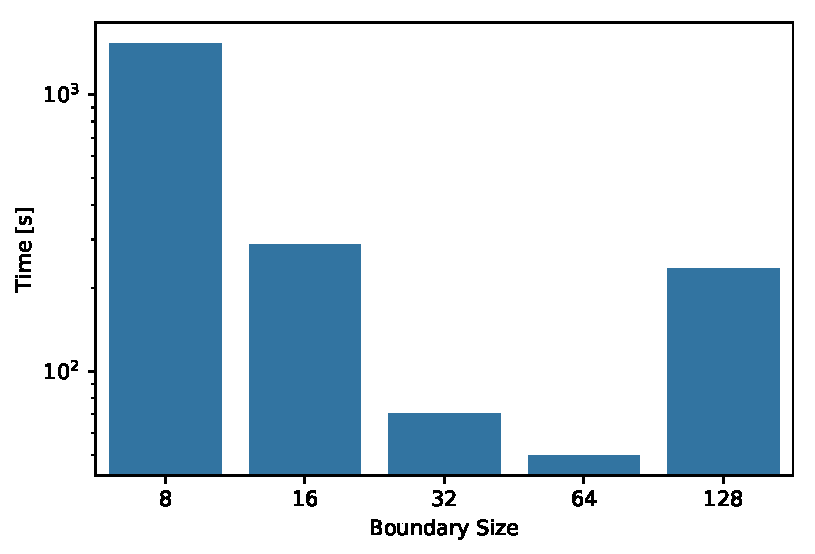
\includegraphics[width=0.6\textwidth]{figs/bm_size_tesla.pdf} 
%\includegraphics[scale=1]{input/ircad_comparison.pdf} 
\caption{Time requirements of LAR-SURF filter used on artificial with different size of boundary matrix}
\label{fig:bm_size_tesla}
\end{figure}



To compare time requirements of LAR-SURF with Marching Cubes implemented in Python we performed experiment on Ircadb dataset \cite{ircad}. Dataset contain 20 Computed Tomography images (see table \ref{tab:ircad1}) with xy-resolution from 0.56 mm to 0.87 mm and z-resolution from 1.0 mm to 4.0 mm. The number of slices is each series varies from 74 to 260 and size of each slice is $512\times512$. Dataset contain manually segmented liver, portal vein and other structures. We performed surface extraction of liver with Marching Cubes and LAR-SURF. Time required for computation can be seen on figure \ref{fig:ircad_comparison}. 

Based on t-test with $\alpha=0.99$, $p=\num[]{8.735e-24}$ and 
$s=\num[]{-16.67}$ it can be shown that the mean of time consumed by LAR-SURF is significantly lower from time consumed by Marching Cubes.


\begin{figure}
\centering
\includegraphics[width=0.99\textwidth]{figs/ircad_comparison.pdf} 
%\includegraphics[scale=1]{input/ircad_comparison.pdf} 
\caption{Time requirements of LAR-SURF filter and Marching Cubes on Ircad dataset. Error bars shows the 95\% confidence interval}
\label{fig:ircad_comparison}
\end{figure}




\section{Examples}\label{sec:examples}




\begin{figure}
\centering
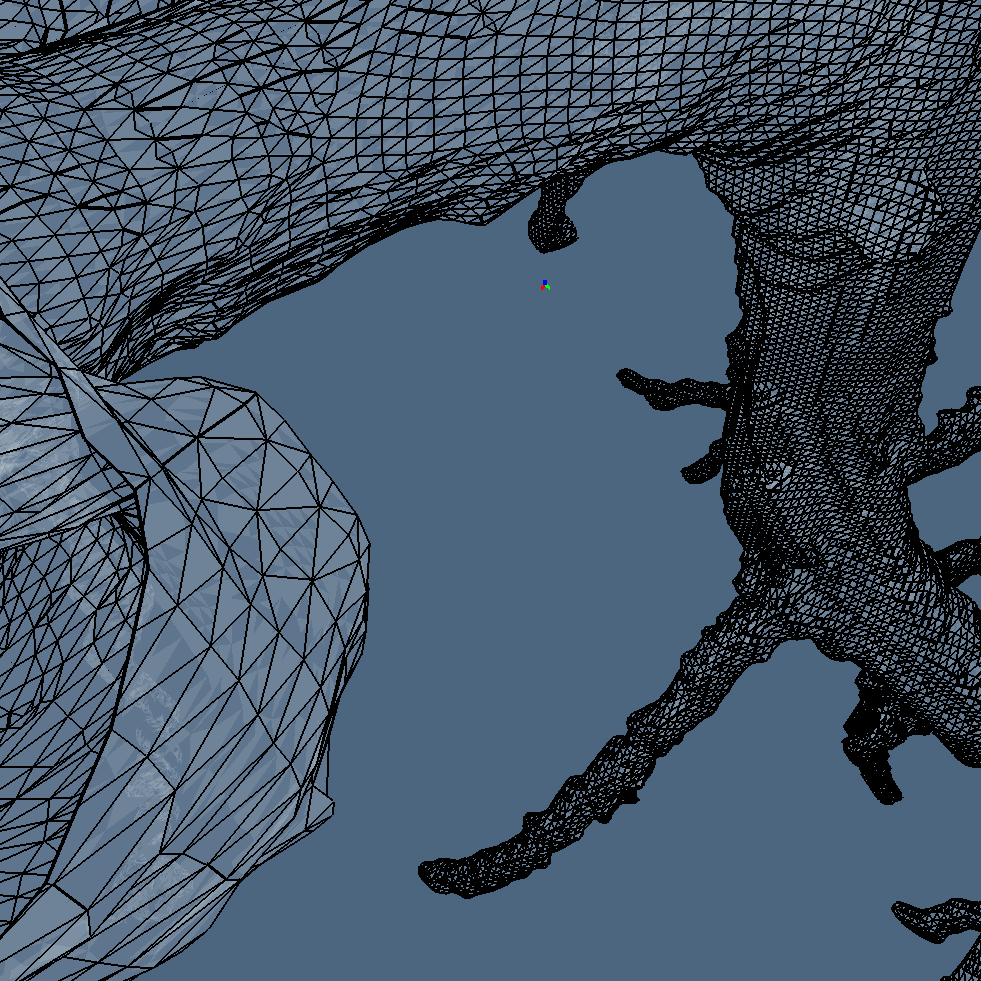
\includegraphics[width=0.4\textwidth]{figs/porta_smoothing_1.png} 
\vspace{0.05\textwidth}
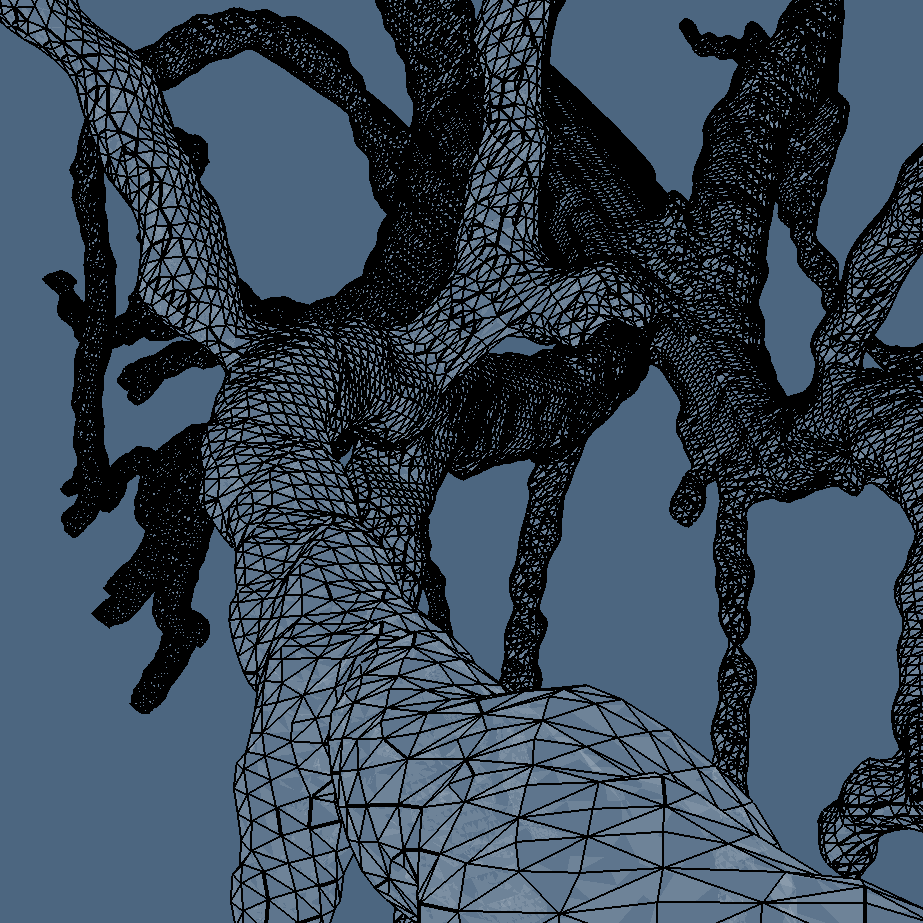
\includegraphics[width=0.4\textwidth]{figs/porta_smoothing_2.png} 
%\includegraphics[scale=1]{input/ircad_comparison.pdf} 
\caption{Triangulated isosurface of portal vein calculated with LAR-SURF}
\label{fig:example_porta}
\end{figure}
\section{Conclusion}\label{sec:conclusion}




\appendix
\section{Appendix}
\subsection{Symbol list}

\begin{description}
\item[$\mathcal{I}$]  three-dimensional medical image

\item[$\ell_1, \ell_2, \ell_3$]  dimensions of image

\item[$\mathcal{S}$]  segment: a subset of voxels from image segmentation

\item[$\mathcal{B}$] 3D image block

\item[$size$] lateral dimension of cubic block $\mathcal{B}$

\item[$n$]	number of blocks $\mathcal{B}$ (jobs) in $\mathcal{I}$

\item[[$\partial_\mathcal{B}$] ]  boundary matrix for block $\mathcal{B}$

\item[$C_p$] linear (vector) space of $p$-chains

\item[$\nu\in C_p$] $p$-chain

\item[[$\nu$]] coordinate representation (binary vector) of  $\nu$

\item[$\E^3$] Euclidean 3-space
\end{description}


\subsection{Definitions}
\begin{description}

\item[Boundary model] Closed manifold surface of the boundary of a solid model

\item[CSC]  Compressed Sparse Column format for sparse matrices

\item[Global coordinates]  Integer linear coordinates of $\mathcal{I}$

\item[Local coordinates] Integer linear coordinates of $\mathcal{B}$

\item[Cartesian coordinates] Integer triples $(i,j,k)$ one-to-one with voxels

\item[Voxels] Individual elements in 3D image (3-cells)

\item[$p$-chain] Formal linear combination of $p$-cells with coefficients in $\{0,1\}$

\item[Coord. repr.]  Binary vector (for $p$-chains) or binary matrix (for chain operators)

\item[Quad]	Geometric quadrilateral; convex polygon with four vertices

\item[Foreground voxel] Individual element of a segment $\mathcal{S}$

\item[Segment]	Subset of voxels resulting from image segmentation
\end{description}

\subsection{Dataset Ircad}

\begin{table}
\begin{tabular}{rrrrrr}
\toprule
 ID &  z-resolution [mm] &  xy-resolution [mm] &  obj. voxels &  size xy &  size z \\
\midrule
  1 &               1.60 &            0.570000 &      2865131 &      512 &     129 \\
  2 &               1.60 &            0.782000 &      1648024 &      512 &     172 \\
  3 &               1.25 &            0.625000 &      2375079 &      512 &     200 \\
  4 &               2.00 &            0.742188 &      1132427 &      512 &      91 \\
  5 &               1.60 &            0.782000 &      2124505 &      512 &     139 \\
  6 &               1.60 &            0.782000 &      1828493 &      512 &     135 \\
  7 &               1.60 &            0.782000 &      1461944 &      512 &     151 \\
  8 &               1.60 &            0.561000 &      3215090 &      512 &     124 \\
  9 &               2.00 &            0.873047 &      1265420 &      512 &     111 \\
 10 &               1.60 &            0.736000 &      1871804 &      512 &     122 \\
 11 &               1.60 &            0.720000 &      1692716 &      512 &     132 \\
 12 &               1.00 &            0.679688 &      3341433 &      512 &     260 \\
 13 &               1.60 &            0.671000 &      2063109 &      512 &     122 \\
 14 &               1.60 &            0.720000 &      1633641 &      512 &     113 \\
 15 &               1.60 &            0.782000 &      1389572 &      512 &     125 \\
 16 &               1.60 &            0.698000 &      2717185 &      512 &     155 \\
 17 &               1.60 &            0.743000 &      2106497 &      512 &     119 \\
 18 &               2.50 &            0.742188 &      1220564 &      512 &      74 \\
 19 &               4.00 &            0.703125 &       583208 &      512 &     124 \\
 20 &               2.00 &            0.808594 &      1359697 &      512 &     225 \\
\bottomrule
\end{tabular}

\label{tab:ircad1}
\end{table}

\begin{table}
\begin{tabular}{lrrrrr}
\toprule
{} &  z-resolution [mm] &  xy-resolution [mm] &   obj. voxels &  size xy &      size z \\
\midrule
% count &           20.00000 &           20.000000 &  2.000000e+01 &     20.0 &   20.000000 \\
min   &            1.00000 &            0.561000 &  5.832080e+05 &    512.0 &   74.000000 \\
mean  &            1.77750 &            0.725141 &  1.894777e+06 &    512.0 &  141.150000 \\
50\%   &            1.60000 &            0.739094 &  1.760604e+06 &    512.0 &  127.000000 \\
% std   &            0.60273 &            0.077233 &  7.206126e+05 &      0.0 &   44.088756 \\
% 25\%   &            1.60000 &            0.693422 &  1.382103e+06 &    512.0 &  121.250000 \\
% 75\%   &            1.70000 &            0.782000 &  2.187148e+06 &    512.0 &  152.000000 \\
max   &            4.00000 &            0.873047 &  3.341433e+06 &    512.0 &  260.000000 \\
\bottomrule
\end{tabular}

\label{tab:ircad2}
\end{table}

\clearpage{}
\bibliographystyle{alpha}
\bibliography{library,TSAS-2019}

\end{document}
